\documentclass[12pt,oneside,a4paper]{book} % This style for A4 format.

%Packages
\usepackage{ecproject}
\usepackage{graphicx}
\usepackage{tikz}
\usetikzlibrary{calc}
\usepackage[a4paper, margin=1in]{geometry}
\usepackage{float}
\usepackage{qrcode}
%%%Page related
\usepackage{fancyhdr} % for header & footer
\usepackage[hidelinks]{hyperref}
\usepackage[toc, nonumberlist]{glossaries} %For Glossaries - to be loaded only after hyperref package
%\ifIndentPara
\usepackage{indentfirst}
%\fi
\usepackage{setspace}
%%%Table Related
%\usepackage{booktabs}
%\usepackage{makecell}
%\usepackage{multirow}
%\usepackage{multicol}


%Document settings
\title{Improvised visual summarizer using denoising algorithm}
%%%%%%%%%%%%%%%Minor (or) Major report%%%%%%%%%%%%%%%
%Uncomment \MinorProject line, if the report is for Minor project.
\MinorProject
%%%%%%%%%%%%%%%%%%%%%%%%%%%%%%%%%%%%%%%%%%%%%%
%%%Student Details%%%
\stuNameA{Sahana K S}
\stuUSNA{1RV17EC190}
\stuNameB{Rakshata Karlingannavar}
\stuUSNB{1RV17EC119}
\stuNameC{Roshni Sen}
\stuUSNC{1RV17EC128}
%\stuNameD{Subrahmanya K N}
%\stuUSND{1RV16EC007}

%%%Internal Guide%%%%
\guideNameA{Mr. Subrahmanya K N}
\guideDesignationA{Assistant Professor}
\guideDeptA{Dept. of ECE}
\guideOrgA{RV College of Engineering}

%%%External Guide%%%%
%\guideNameB{Dr. Ramavenkateshwaran}
%\guideDesignationB{Assistant Professor}
%\guideDeptB{Dept. of ECE}
%\guideOrgB{RV College of Engineering}

%\guideNameC{Dr. Ramavenkateshwaran}
%\guideDesignationC{Assistant Professor}
%\guideDeptC{Dept. of ECE}
%\guideOrgC{RV College of Engineering}

\panelMemberA{Dr.Govinda Raju M.}
\panelMemberDesigA{Assistant Professor}
\panelMemberB{Dr. Ramavenkateswaran.N.}
\panelMemberDesigB{Assistant Professor}

\Department[ECE]{Electronics and Communication Engineering}

\HOD{Dr. K S Geetha}
\Principal{Dr. K. N. Subramanya}

\academicYear{2020-2021}

\QRurl{}
%\QRurl{https://drive.google.com/open?id=1jm-POmuq-ZZ1tT5m-xAdCDRnwvLZH8q-}
%%%%%%%%%%%%%%%%%%%For PG program%%%%%%%%%%%%%%%%%%%
%%%Uncomment \pgProgram command and define appropriate values for \MastersIn{} and \pgProgramName{}

%\pgProgram%
\MastersIn[M.Tech]{Master of Technology}
\pgProgramName{VLSI Design \& Embedded Systems}

%%%%%%%%%%%%%%%%%%Draft report%%%%%%%%%%%%%%%%%%
\DraftCopy
%%%%%%%%%%%%%%%%%%%%%%%%%%%%%%%%%%%%%%%%%%%%%%

%%%%%%%%%%%%%%%%%%Acronyms%%%%%%%%%%%%%%%%%%
\newglossary[sym]{symbolList}{sym1}{sym2}{List of Symbols}
\makeglossaries
%Acronyms
\loadglsentries{./AuxFiles/Glossaries}
\renewcommand{\glspostdescription}{}% To remove dot at the end
%%%%%%%%%%%%%%%%%%%%%%%%%%%%%%%%%%%%%%%%%%%%%%

%%%%%%%%%%%%%%Bibliography%%%%%%%%%%%%%%%%%%%%%
\usepackage[backend=biber,style=ieee]{biblatex}
%If backend is set to bibtex, then configure texmaker Bi(La)Tex with "bibtex %"
\addbibresource{./AuxFiles/ProjectBib.bib}%Add bib file with extention
%%%%%%%%%%%%%%%%%%%%%%%%%%%%%%%%%%%%%%%%%%%%%%

%%%%%%%%%%%%%%%%WaterMark%%%%%%%%%%%%%%%%%%%%%
%%Use it only after Biblatex
\usepackage[printwatermark]{xwatermark}
\newwatermark[allpages,color=gray!50,angle=0,scale=2,xpos=0,ypos=0]{
\includegraphics[width=0.3\textwidth]{Figures/RVlogoVecW}}
%\usepackage{background}
%\backgroundsetup{scale=1, angle=0, firstpage = true, opacity=1, contents={
%\begin{tikzpicture}[remember picture, overlay]
%\node at ([yshift=0pt, xshift=0pt]current page.center){\includegraphics[width=0.3\textwidth]{Figures/RV_logoVecW}};
%\end{tikzpicture}
%}}
%%%%%%%%%%%%%%%%%%%%%%%%%%%%%%%%%%%%%%%%%%%%%%
\begin{document}
\maketitle
%\pagestyle{empty}
\newpage
\begin{spacing}{1.5}
%%ecproject package is created by P Narashimaraja, Assistant Professor, ECE, RVCE
%Border
\begin{tikzpicture}[remember picture, overlay]
  \draw[line width = 4pt] ($(current page.north west) + (0.75in,-0.75in)$) rectangle ($(current page.south east) + (-0.75in,0.75in)$);
\end{tikzpicture}
\thispagestyle{empty}
\vspace{-1cm}
\begin{center}
\Large\textbf{RV College of Engineering\textsuperscript{\small\textregistered}, Bengaluru} \par
\large{(\textit{Autonomous institution affiliated to VTU, Belagavi})} \par
\large\textbf{Department of \printDepartmentLF}\\
.\hspace{2cm}\\

\includegraphics[width=4cm]{Figures/RV_logoVec}\par
\Large\textbf{\underline{CERTIFICATE}} \par
\end{center}
%\begin{minipage}[b]{\linewidth}
%\large
\begin{spacing}{1.5}
\noindent Certified that the \ifMinor{minor\;}\else{ major\;}\fi project work titled \textbf{\textit{\printTitle}} is carried out by
\ifPG{%
\textbf{\printStuNameA} (\textbf{\printStuUSNA}) who is  bonafide student 
}
\else{
\ifStuNameDUsed{%
\textbf{\printStuNameA } (\textbf{\printStuUSNA}), \textbf{\printStuNameB } (\textbf{\printStuUSNB}), \textbf{\printStuNameC } (\textbf{\printStuUSNC}) and \textbf{\printStuNameD } (\textbf{\printStuUSND})  who are bonafide students 
}\else{% 
\ifStuNameCUsed{%
\textbf{\printStuNameA } (\textbf{\printStuUSNA}), \textbf{\printStuNameB } (\textbf{\printStuUSNB}) and \textbf{\printStuNameC } (\textbf{\printStuUSNC})  who are bonafide students 
}\else{%
\ifStuNameBUsed{%
\textbf{\printStuNameA} (\textbf{\printStuUSNA}) and \textbf{\printStuNameB} (\textbf{\printStuUSNB})  who are bonafide students 
}\else{%
\textbf{\printStuNameA} (\textbf{\printStuUSNA}) who is  bonafide student 
}
\fi
}\fi
}\fi
}\fi
of RV College of Engineering, Bengaluru, in partial fulfillment of the requirements for the degree of  \ifPG \textbf{\printMastersInLF} in \textbf{\printMastersPrgName} \else\textbf{Bachelor of Engineering} in \textbf{\printDepartmentLF} \fi of the Visvesvaraya Technological University, Belagavi during the year \printAcadYear. It is certified that all corrections/suggestions indicated for the Internal Assessment have been incorporated in the \ifMinor{minor\;}\else{major\;}\fi project report deposited in the departmental library. The \ifMinor{minor\;}\else{ major\;}\fi project report has been approved as it satisfies the academic requirements in respect of \ifMinor{minor\;}\else{ major\;}\fi project work prescribed by the institution for the said degree.\\ \par
\end{spacing}

\begin{table}[H]
\centering
\resizebox{1\textwidth}{!}{%
\begin{tabular}{ccc}
\large Signature of Guide &\large Signature of Head of the Department &\large Signature of Principal\\
& &\\
\large\printGuideNameA & \large\printHOD & \large\printPrincipal\\
& & \\
\end{tabular}%
}
\end{table}

\begin{table}[H]
\centering
%\resizebox{\textwidth}{!}{%
\begin{tabular}{lccp{6cm}cc}
&&&\textbf{External Viva}&&\\
&&&&&\\
&Name of Examiners &&& & Signature with Date\\
&&&&&\\
1.&&&&&\\
&&&&&\\
2.&&&&&\\
\end{tabular}%
%}
\end{table}
%\pagebreak
\newpage
%%ecproject package is created by P Narashimaraja, Assistant Professor, ECE, RVCE
%%Border
\begin{tikzpicture}[remember picture, overlay]
  \draw[line width = 4pt] ($(current page.north west) + (0.75in,-0.75in)$) rectangle ($(current page.south east) + (-0.75in,0.75in)$);
\end{tikzpicture}

\thispagestyle{empty}

\begin{center}
\Large\textbf{\underline{DECLARATION}} \par
\end{center}


\noindent \ifPG I \else \ifStuNameBUsed We\else I\fi\fi, \textbf{\printStuNameA} \ifPG \else\ifStuNameBUsed  \ifStuNameCUsed ,$\,$ \else{$\,$ and $\,$}\fi \textbf{\printStuNameB} \ifStuNameCUsed  \ifStuNameDUsed ,$\,$ \else{$\,$ and $\,$}\fi \textbf{\printStuNameC}$\,$ \ifStuNameDUsed and $\,$ \textbf{\printStuNameD}$\,$ \fi \fi \fi \fi students of \ifPG fourth \else \ifMinor{seventh\;}\else{eighth\;}\fi \fi semester \ifPG \printMastersInSF\, in \printMastersPrgName \else B.E.\fi, Department of \printDepartmentLF, RV College of Engineering, Bengaluru, hereby declare that the \ifMinor{minor\;}\else{ major\;}\fi project titled `\textbf{\printTitle}' has been carried out by \ifStuNameBUsed us \else me \fi and submitted in partial fulfilment for the award of degree of \ifPG \textbf{\printMastersInLF} in \textbf{\printMastersPrgName} \else\textbf{Bachelor of Engineering} in \textbf{\printDepartmentLF} \fi during the year \printAcadYear.\\ \par

\noindent Further \ifPG I \else\ifStuNameBUsed we \else I \fi \fi declare that the content of the dissertation has not been submitted previously by anybody for the award of any degree or diploma to any other university.\\ \par

\noindent \ifPG I \else\ifStuNameBUsed We \else I \fi \fi also declare that any Intellectual Property Rights generated out of this project carried out at RVCE will be the property of RV College of Engineering, Bengaluru and we will be one of the authors of the same.

\vspace{1cm}
\noindent Place: Bengaluru\par
\vspace{0.5cm}
\noindent Date: \par

\vspace{2cm}
\begin{table}[H]
\centering
%\resizebox{\textwidth}{!}{%
\begin{tabular}{llcp{5cm}cc}
&&&&&\\
&&&&&\\
&Name  &&& Signature& \\
&&&&&\\
1.&\printStuNameA (\printStuUSNA)&&&&\\
&&&&&\\
\ifPG% 
\else%
\ifStuNameBUsed%
2.&\printStuNameB (\printStuUSNB)&&&&\\
&&&&&\\
\else%
\fi%
\ifStuNameCUsed%
3.&\printStuNameC (\printStuUSNC)&&&&\\
&&&&&\\
\else%
\fi%
\fi%
\end{tabular}%
%}
\end{table}
%\pagebreak


\newpage
%%ecproject package is created by P Narashimaraja, Assistant Professor, ECE, RVCE.
%%Border
\begin{tikzpicture}[remember picture, overlay]
  \draw[line width = 4pt] ($(current page.north west) + (0.75in,-0.75in)$) rectangle ($(current page.south east) + (-0.75in,0.75in)$);
\end{tikzpicture}
\thispagestyle{empty}

\begin{center}
%.\hspace{1cm}\\ \par
\Large\textbf{\underline{ACKNOWLEDGEMENT}} \par
\end{center}

\ifPG I am \else
\ifStuNameBUsed We are \else I am \fi\fi indebted to \ifPG my \else\ifStuNameBUsed our \else my \fi\fi guide, \textbf{\printGuideNameA}, \printGuideDesigA, \printGuideOrgA$\,.$ for the wholehearted support, suggestions and invaluable advice throughout \ifPG my \else\ifStuNameBUsed our \else my \fi\fi project work and also helped in the preparation of this thesis.\\ \par

\ifPG I \else \ifStuNameBUsed We \else I \fi\fi also express our gratitude to \ifPG my \else\ifStuNameBUsed our \else my \fi\fi  panel members \textbf{\printPanelMemberA}, \printPanelMemberDesigA $\,$ and \textbf{\printPanelMemberB}, \printPanelMemberDesigB , Department of \printDepartmentLF\, for their valuable comments and suggestions during the phase evaluations. \\ \par

\ifPG My \else \ifStuNameBUsed Our \else My \fi\fi sincere thanks to \textbf{\printHOD}, Professor and Head, Department of \printDepartmentLF, RVCE for the support and encouragement.\\ \par

\ifPG I \else \ifStuNameBUsed We \else I \fi\fi express sincere gratitude to our beloved Principal, \textbf{\printPrincipal} for the appreciation towards this project work.\\ \par

\ifPG I \else\ifStuNameBUsed We \else I \fi\fi thank all the teaching staff and technical staff of \printDepartmentLF\, department, RVCE for their help.\\ \par 

Lastly, \ifPG I \else\ifStuNameBUsed we \else I \fi\fi take this opportunity to thank \ifPG my \else\ifStuNameBUsed our \else my \fi\fi family members and friends who provided all the backup support throughout the project work.\\ \par

%\pagebreak
\newpage
\pagenumbering{roman}
\chapter*{Abstract}
\addcontentsline{toc}{chapter}{Abstract}\vspace{-1cm}
%Border
\begin{tikzpicture}[remember picture, overlay]
  \draw[line width = 4pt] ($(current page.north west) + (0.75in,-0.75in)$) rectangle ($(current page.south east) + (-0.75in,0.75in)$);
\end{tikzpicture}


% Highlights of significant contributions: One page with 3 to 4 paragraphs\\

% Paragraph 1: Importance of Topic, Present shortcomings in performance or computation etc, issues involved in the shortcomings, short on what is done in this report addressing shortcomings

Technology is an evolutionary process that has gained traction in business, academia and government in the recent years. Lectures in classrooms have advanced to the extent of using smart-boards and smart-classrooms. However, there exists an absence of any technological advancement regarding jotting down notes during a presentation or seminar. Our project aims to aid the attendees of any seminar, presentation or lecture in recording vital information in the form of concise notes. The main shortcoming was lack of GPU and limited RAM availability. Due to this, denoising autoencoder had to be trained on very few images. This might make the model vulnerable to overfitting, hence leading to model memorising the training images and producing very high training accuracy and very low validation accuracy. This was avoided by using L2 regularization which avoids overfitting of the model by penalising the weights that are very large.\\

% Paragraph 2 Objectives of this work, short on algebraic methods used and formulations achieved, computational procedures developed. 

The objectives of our project were to develop and train a denoising autoencoder to deblur the input image, to build an object detection model to detect text from the deblurred image and finally, to extract the detected text and summarize it using extractive summarization. By doing so, we will achieve the goal of our visual summarizer, that is to generate concise notes from any presentation or lecture.\\


% Paragraph 3: Description of simulation procedure including SW tools used and choice of test cases. Short on results achieved and significant highlights of improvements if any.

The software tools used for our project include PyCharm, Google Colab and LabelImg. Software libraries used to train machine learning models are Tensorflow, Keras, \acrshort{ocv}, PyTesseract, NLTK (Natural Language Processing Toolkit), matplotlib, pandas and numpy to name a few. We have achieved a very efficient reconstruction of blurred images and, successfully implemented text extraction and summarization on them. Model accuracies can be further improved by increasing the size of the image dataset and training for more number of epochs.

\pagebreak
\end{spacing}
\newpage
\pagestyle{fplain}
\begin{spacing}{1.5}
	\tableofcontents	
\end{spacing}
\newpage
\begin{spacing}{1.5}
	\cleardoublepage
	\addcontentsline{toc}{chapter}{\listfigurename}
	\listoffigures	
\end{spacing}
\newpage
\begin{spacing}{1.5}
	\cleardoublepage
	\addcontentsline{toc}{chapter}{\listtablename}
	\listoftables	
\end{spacing}
\newpage
\printglossary[type=\acronymtype, title= Abbreviations, toctitle=Abbreviations]
\newpage
% \printglossary[type=symbolList, title= List of Symbols, toctitle=List of Symbols]

\mainmatter
\pagestyle{mplain}
\glsresetall
\begin{spacing}{1.5}
%Chapter 1 
\chapter{Introduction to Analog and Digital converters}
Every chapter should start with an introduction paragraph. This paragraph should brief about the flow of the chapter. This introduction can be limited within 4 to 5 sentences. The chapter heading should be appropriately modified (a sample heading is shown for this chapter).
\section[Introduction]{\textbf{Introduction}}
The title of the project can be introduced in this section. This section should neatly elaborate the context of the project, the relevance of the area chosen and the title. You can bring a brief history and arrive at the title of the project. Use appropriate number of paragraphs within this section. 

You are allowed to use figures or diagrams which can help in introducing the topic acknowledging the source. For example , if you are introducing a particular topic, an appropriate figure can be used. The figure should be referenced in the text as Figure. \ref{fig:universe} 
\begin{figure}[htb]
\centering
	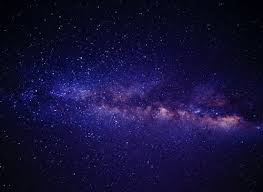
\includegraphics[scale=1]{Figures/universe}	
	\caption{Sample picture of universe }
	\label{fig:universe}
\end{figure}

These guidelines are provided to formally expose you to the various ethical and technical issues involved in writing up your work and the format you are required to adhere to while submitting your project report.

\section[Motivation]{\textbf{Motivation}}

Brief the motivation of selecting your project title. You can elaborate the challenges in the specific area, relevance and importance of the chosen topic. 

\section[Problem statement]{\textbf{Problem statement}}

Define the problem statement in this section, in one paragraph.

\section[Objectives]{\textbf{Objectives}}
The objectives of the project are
\begin{enumerate}
\item To design a pipelined ADC for audio frequency range
\item List all the objectives in the above format , starting with "To"
\item Limit the number of objectives to a maximum of three
\end{enumerate}

\section[Literature Review]{\textbf{Literature Review}}

A literature review is a text of a scholarly paper, which includes the current knowledge including substantive findings, as well as theoretical and methodological contributions to a particular topic. Literature reviews are secondary sources, and do not report new or original experimental work. Most often associated with academic-oriented literature, such reviews are found in academic journals, and are not to be confused with book reviews that may also appear in the same publication. Literature reviews are a basis for research in nearly every academic field . A narrow-scope literature review may be included as part of a peer-reviewed journal article presenting new research, serving to situate the current study within the body of the relevant literature and to provide context for the reader. In such a case, the review usually precedes the methodology and results sections of the work.

\subsection{Sample}
The main types of literature reviews are: evaluative, exploratory, and instrumental. A fourth type, the systematic review, is often classified separately, but is essentially a literature review focused on a research question, trying to identify, appraise, select and synthesize all high-quality research evidence and arguments relevant to that question. A meta-analysis is typically a systematic review using statistical methods to effectively combine the data used on all selected studies to produce a more reliable result.
\subsubsection[Review types]{\textbf{Review types}}

The main types of literature reviews are: evaluative, exploratory, and instrumental. A fourth type, the systematic review, is often classified separately, but is essentially a literature review focused on a research question, trying to identify, appraise, select and synthesize all high-quality research evidence and arguments relevant to that question. A meta-analysis is typically a systematic review using statistical methods to effectively combine the data used on all selected studies to produce a more reliable result.


\subsubsection[Process and product]{\textbf{Process and product}}

Distinguish between the process of reviewing the literature and a finished work or product known as a literature review. The process of reviewing the literature is often ongoing and informs many aspects of the empirical research project. All of the latest literature should inform a research project. Scholars need to be scanning the literature long after a formal literature review product appears to be completed.

\subsubsection{\textbf{Page limitation}}

A careful literature review is usually 15 to 30 pages and could be longer. The process of reviewing the literature requires different kinds of activities and ways of thinking and link the activities of doing a literature review with Benjamin Bloom’s revised taxonomy of the cognitive domain (ways of thinking: remembering, understanding, applying, analysing, evaluating, and creating).

This section should contain the review of the literature in the past.You should review a minimum of 10 papers from standard reference journals. Kindly avoid local conference papers and papers from predatory journals. Kindly consult with your guide and finalize papers to be considered for review before adding in this section.Report the major observations and findings from each paper in one paragraph in the format given below.

 proposed various techniques for adders and multipliers.Add the reference papers to the bibliography section using Jabref and cite it here using the instructions given in further chapters.


\subsubsection{\textbf{Plagiarism}}

To use someone else's exact words without quotation marks and appropriate credit, or to use the unique ideas of someone else without acknowledgement, is known as plagiarism. In publishing, plagiarism is illegal; in other circumstances, it is, at the least, unethical. You may quote or paraphrase the words or ideas of another if you document your source. Although you need not enclose the paraphrased material in quotation marks, you must document the source. 

Paraphrased ideas are taken from someone else whether or not the words are identical. Paraphrasing a passage without citing the source is permissible only when the information paraphrased is common knowledge in a field. (Common knowledge refers to historical, scientific, geographical, technical, and other type of information on a topic readily available in handbooks, manuals, atlases and other references). 

\subsubsection{How to add Reference}
Use \texttt{Jabref} which will help in adding the reference in a separate file, from which one can use \verb|\citep\{\}| command to add reference. A sample, referring to a textbook would look something like this,\cite{Razavi2000}.

\section[Brief Methodology of the project]{\textbf{Brief Methodology of the project}}
Discuss about the methodology you identified to execute the objectives of your project in brief. Methodology is a system of practices, techniques, procedures, and rules used to execute a particular project. You can elaborate the methodology in a later chapter. Here you can present in the form of a flow diagram and explain the methodology in a paragraph.

\section[Assumptions made / Constraints of the project]{\textbf{Assumptions made / Constraints of the project}}

List the assumptions made for the execution of the project in this section. You can also elaborate on the major constraints of the project. This section should clearly state under what conditions your project is valid. It is mandatory to have this section in your project report.

\section[Organization of the report]{\textbf{Organization of the report}}

This report is organized as follows. Write the discussions in each chapter. A sample is as follows.
\begin{itemize}
\item Chapter 2 discusses the fundamentals of ADC and the performance parameters for evaluation.
\end{itemize}

In a similar way, write briefly about each chapter in one or two sentences.

%Chapter 2
\chapter{Convolutional Neural Networks (CNN)}

In Convolutional Neural Networks, the goal is to provide an image as an input and generate an output that determines the probability of the image belonging to a certain class. This chapter discusses the fundamentals of CNN as well as its various layers, i.e the Convolutional Layer, the Pooling Layer and the Fully Connected Layer.
\section{Introduction to \acrlong{cnn}}

Artificial Intelligence has contributed in a monumental manner to bridge the gap between humans and computer abilities. To make great things possible, researchers work on various facets of the area, the domain of Computer Vision being one of several such fields. The goal for this field is to allow machines to view the world as humans do, interpret it in a similar way and even use information for a variety of tasks, such as recognition of images and videos, reconstruction of media, recommendation systems, processing of natural languages, and so on. With time, the advances in Computer Vision with Deep Learning have been developed and refined, predominantly through a specific algorithm, a Convolutional Neural Network.

A Convolutional Neural Network (ConvNet/\acrshort{cnn}) is a deep learning algorithm that can take an input image, assign significance to various aspects/objects in the image and be able to distinguish one from the other. In comparison to other classification algorithms, the pre--processing required in a CNN is much lower. In \acrshort{cnn}, filters are not hand-engineered -- with enough training, they have the ability to learn these filters. 

The architecture of Convolutional Neural Networks differs from that of regular Neural Networks. In case of regular Neural Networks, an  is transformed by passing it through multiple hidden layers where each layer consists of a set of neurons and is entirely connected to all neurons in the layer before, following which there is a final fully-connected layer — the output layer — that represents the predictions. There is a slight difference in case of Convolutional Neural Networks. Here, the layers are organised in 3 dimensions: width, height and depth. Further, the neurons in one layer do not connect to all the neurons in the next layer but only to a small region of it. Ultimately, the final output will be reduced to a single vector of probability scores, organized along the depth dimension.
\section{Working of \acrlong{cnn}}
A \acrshort{cnn} has several layers for processing an image which are discussed below.
\subsection{Convolution Layer}
This is the first layer to extract features from an input image. An image is nothing but a matrix of pixel values. Convolution preserves the relationship between pixels by learning image features using small squares of input data. It is a mathematical operation that takes two inputs such as image matrix and a filter or kernel to produce a feature map. Convolution is executed by sliding the filter over the input. At every location, a matrix multiplication is performed between the image matrix and the filter matrix and the result is summed onto the feature map as shown in figures \ref{fig:imagemat} and \ref{fig:outputmat}. 

% \ref{fig:object} 
\begin{figure}[H]
\centering
	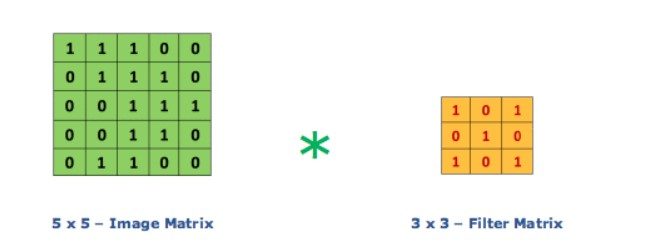
\includegraphics[scale=1]{Chapter2/img_mat_mul_kernel_filter_matrix.jpg}	
	\caption{Image matrix multiplied with kernel or filter matrix}
	\label{fig:imagemat}
\end{figure}
\begin{figure}[H]
\centering
	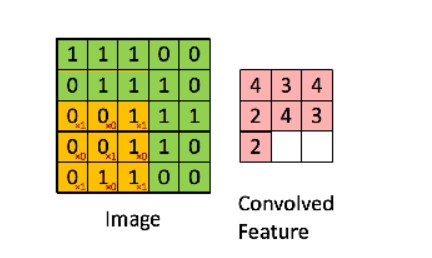
\includegraphics[scale=1]{Chapter2/output_mat.jpg}	
	\caption{Output matrix}
	\label{fig:outputmat}
\end{figure}
% INSERT IMGMATMUL AND OUTPUTMAT IMAGES HERE. 

Operations such as edge detection, blur and sharpen can be achieved by convolution of an image with different filters.


\subsection{Pooling Layer}
When the images are too large, pooling layers can reduce the number of parameters. Spatial pooling, also called subsampling or downsampling, reduces the dimensionality of each map but retains important information. Spatial pooling can be of several types:
\begin{enumerate}
    \item Max Pooling
    \item Average Pooling
    \item Sum Pooling
\end{enumerate}
Max Pooling returns the maximum value from the portion of the image covered by the kernel. Average Pooling returns the average of all the values from the portion of the image covered by the Kernel. Sum of all elements in the feature map is called Sum Pooling.

\begin{figure}[H]
\centering
	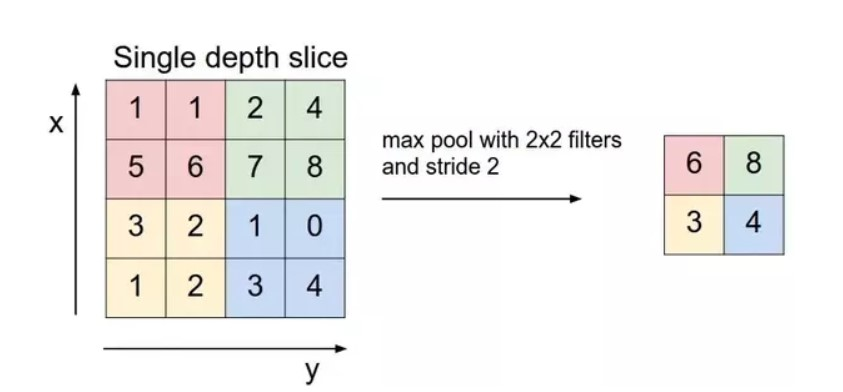
\includegraphics[scale=1]{Chapter2/max_pooling.jpg}	
	\caption{Max Pooling}
	\label{fig:maxpool}
\end{figure}
% INSERT MAX POOLING IMAGE HERE.

\subsection{Fully Connected Layer}
The input to the fully connected layer is the output from the final Pooling or Convolutional Layer, which is flattened (unroll the output of final (and any) Pooling and Convolutional Layer, which is a 3-dimensional matrix, values into a vector) and then fed into the fully connected layer.

\begin{figure}[H]
\centering
	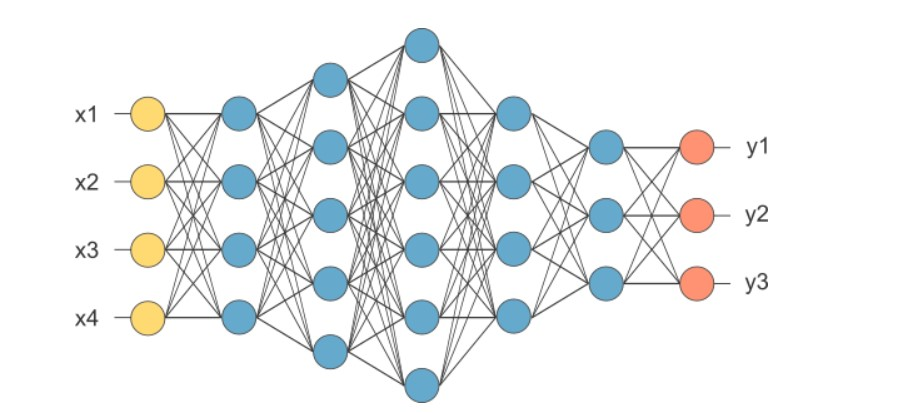
\includegraphics[scale=1]{Chapter2/after_pooling_layer_flattened_as_FC_layer.jpg}	
	\caption{After pooling layer, flattened as FC layer}
	\label{fig:after_pooling}
\end{figure}
% INSERT AFTERPOOLINGFLATTENED..FC IMAGE HERE.

In the above diagram, the feature map matrix will be converted as vector (x1, x2, x3, ...). With the Fully Connected Layers, we combine these features together to create a model. Finally, we have an activation function such as softmax or sigmoid to classify the outputs as  car, truck, cat, dog, etc.

\section{Other parameters associated with \acrshort{cnn} layers}

\subsection{Stride} 
It is the number of pixels shifts over the input matrix. We move the filter 1 pixel at a time when the stride is 1. We move the filter 2 pixels at a time when the stride is 2 and so on. Figure \ref{fig:stride} shows convolution would work with a stride of 2.

\begin{figure}[H]
\centering
	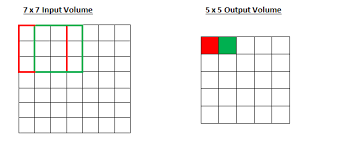
\includegraphics[scale=1]{Chapter2/stride.png}
	\caption{Stride}
	\label{fig:stride}
\end{figure}
% INSERT STRIDE IMAGE HERE.

\subsection{Padding}
There are times when the filter does not perfectly fit the input image. In such cases, there are two options:
\begin{enumerate}
    \item Pad the picture with zeros (zero-padding) so that it fits
    \item Drop the part of the image where the filter did not fit. This is called valid padding which keeps only valid part of the image.
\end{enumerate}

\subsection{Non Linear Activation function}
Activation functions are mathematical equations that determine the output of a neural network. The function is attached to each neuron in the network, and determines whether it should be activated (“fired”) or not, based on whether each neuron's input is relevant for the model's prediction. An example for activation function is ReLU (Rectified Linear Unit). ReLU is a non linear activation function defined as ƒ(x) $=$ max(0,x). It will output the input directly if it is positive, otherwise, it will output zero. It has become the default activation function for many types of neural networks since the problem of having negative weights can be avoided as negative values will be scaled to 0.

\begin{figure}[H]
\centering
	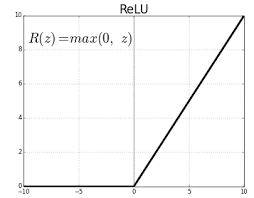
\includegraphics[scale=1]{Chapter2/relu.png}	
	\caption{ReLU activation Function}
	\label{fig:relu}
\end{figure}
% INSERT RELU IMAGE HERE.



% \section{Summary}
In summary, the CNN architecture is as follows. The input image is provided to the convolution layer. Parameters are chosen, filters with strides are applied along with padding, if required. Convolution on the image is performed and a non linear activation is applied to the matrix. Pooling is performed to reduce image dimension. The output of this stage is flattened and fed into a fully connected layer (FC Layer). This layer outputs the class to which the input image belongs.
\begin{figure}[H]
\centering
	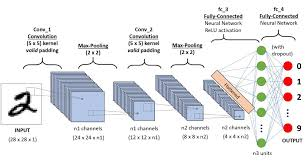
\includegraphics[scale=1.25]{Chapter2/cnn.jpeg}	
	\caption{CNN architecture}
	\label{fig:CNN}
\end{figure}
% INSERT COMPLETE CNN ARCHITECTURE IMAGE HERE.


%Chapter 3
\chapter{Object Detection using Faster R--CNN}

\indent\indent Object detection is a computer vision task that involves predicting where the required objects are in an image. This chapter gives an introduction to object detection. It further gives details on one of the most efficient object detection algorithms, the Faster \acrshort{rcn} model and then gives the summary of the trained object detection model.  
\section{Introduction to Object Detection}
Image Processing is a technique that plays out a couple of assignments in a picture, to generate a picture which is improved or to extricate information that is supportive from it. A kind of sign handling it is, in which info is a picture and yield may be picture or highlights related with that image. In the recent days, image preparing is one of the rapidly creating developments. It shapes focus examine district inside structure and disciplines too of programming building. Picture handling incorporates fundamentally the three accompanying stages, bringing in the picture by means of securing picture instruments, controlling and breaking down the picture and yield in which the end data can be changed picture or report that depends on picture examination. There are couple of types of strategies used for picture preparing explicitly, simple and computerized image handling. Image specialists use few nuts and bolts of comprehension while simultaneously using these visual procedures. Advanced Image handling strategies help in charge of the modernized pictures by using PCs. A library fundamentally focused on current-time computer vision of programming capacities is \gls{ocv}. \gls{ocv} bolsters a few models from profound learning structures like TensorFlow, Torch, PyTorch (subsequent to changing over to an ONNX model) and Caffe as indicated by a characterized rundown of upheld layers. It
advances OpenVisionCapsules, which is a versatile configuration, perfect with every other arrangement.\\
Computer vision is an interdisciplinary field that has been gaining huge amounts of traction in the recent years(since CNN) and self-driving cars have taken centre stage. Another integral part of computer vision is object detection. Object detection aids in pose estimation, vehicle detection, surveillance etc. The difference between object detection algorithms and classification algorithms is that in detection algorithms, we try to draw a bounding box around the object of interest to locate it within the image. Also, you might not necessarily draw just one bounding box in an object detection case, there could be many bounding boxes representing different objects of interest within the image and you would not know how many beforehand.\\
Object detection \cite{8627998} is a computer vision technique which used image processing that allows us to identify and locate objects in an image or video. With this kind of identification and localization, object detection can be used to count objects in a scene and determine and track their precise locations, all while accurately labeling them.\\
Object recognition is a general term to describe a collection of related computer vision tasks that involve identifying objects in digital photographs.
Image classification involves predicting the class of one object in an image. Object localization refers to identifying the location of one or more objects in an image and drawing abounding box around their extent. Object detection combines these two tasks and localizes and classifies one or more objects in an image.\\
As such, we can distinguish between these three computer vision tasks:
\begin{enumerate}
\item Image Classification: Predict the type or class of an object in an image.
\begin{enumerate}
    \item Input: An image with a single object, such as a photograph.
    \item Output: A class label (e.g. one or more integers that are mapped to class labels).
\end{enumerate}
\item Object Localization: Locate the presence of objects in an image and indicate their location with a bounding box.
\begin{enumerate}
    \item Input: An image with one or more objects, such as a photograph.
    \item Output: One or more bounding boxes (e.g. defined by a point, width, and height).
\end{enumerate}
\item Object Detection: Locate the presence of objects with a bounding box and types or classes of the located objects in an image.
\begin{enumerate}
    \item Input: An image with one or more objects, such as a photograph.
    \item Output: One or more bounding boxes (e.g. defined by a point, width, and height), and a class label for each bounding box.
\end{enumerate}
\end{enumerate}
% \ref{fig:object} 
\begin{figure}[H]
\centering
	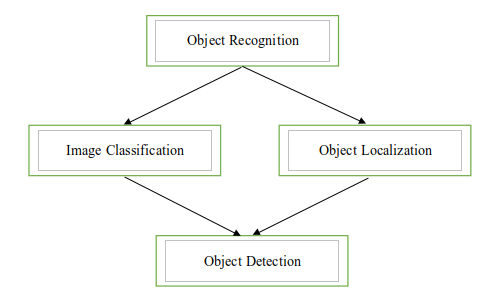
\includegraphics[scale=1]{Figures/object.png}	
	\caption{Object Detection}
	\label{fig:object}
\end{figure}
A naive approach to solve this problem would be to take different regions of interest from the image, and use a CNN to classify the presence of the object within that region. The problem with this approach is that the objects of interest might have different spatial locations within the image and different aspect ratios. Hence, you would have to select a huge number of regions and this could computationally blow up. Therefore, algorithms like \acrshort{rcn}, YOLO etc have been developed to find these occurrences and find them fast.
\section{Introduction to \acrlong{rcn}}
The problem the R--CNN system tries to solve it is to locate objects in an image (object detection). R--CNN “Region-based Convolutional Neural Networks”. The main idea is composed of two steps. 
\begin{enumerate}
    \item First, using selective search, it identifies a manageable number of bounding-box object region candidates (“region of interest” or “RoI”). 
    \item It then extracts CNN features from each region independently for classification.
\end{enumerate}
To make \acrshort{rcn} faster, the training procedure was improved by unifying three independent models into one jointly trained framework and increasing shared computation results, named Fast \acrshort{rcn}. Instead of extracting CNN feature vectors independently for each region proposal, this model aggregates them into one CNN forward pass over the entire image and the region proposals share this feature matrix. Then the same feature matrix is branched out to be used for learning the object classifier and the bounding-box regressor. In conclusion, computation sharing speeds up \acrshort{rcn}. Fast \acrshort{rcn} is much faster in both training and testing time. However, the improvement is not dramatic because the region proposals are generated separately by another model and that is very expensive.\\
An intuitive speedup solution is to integrate the region proposal algorithm into the CNN model. \acrlong{rcn} \cite{wang2017scene} is doing exactly this: construct a single, unified model composed of RPN (region proposal network) and fast R-CNN with shared convolutional feature layers.\\
\acrfull{rcn} is composed of 3 neural networks — Feature Network, Region Proposal Network (RPN), Detection Network.

\section{Software Setup}
\begin{enumerate}
\item Tensorflow: It is an open source stage from start to finish for AI. An exhaustive, biological system of instruments that is adaptable is included in it, network assets and libraries that lets ML to be pushed best in class by scientist and ML fueled applications are effectively assembled and conveyed by engineers.
\item LabelImg tool: LabelImg is a free, open source tool for graphically labeling images. It's written in Python and uses QT for its graphical interface. It is an 
an open-source image labeling tool for training classifiers.
\end{enumerate}

\section{Text Detection model using \acrlong{rcn}}
The object detection was successfully performed using TensorFlow object detection. COCO models provided pre-defined models for object detection. A variety of models with pre-assigned set of initial weights and pre-made architectures allowed flexibility in choosing the models based on training results. The faster{\_}rcnn{\_}v2{\_}coco model \cite{bhat2018cost} offered a considerably greater accuracy. Here the \acrshort{rcn} \cite{8627998} model applies high-capacity convolutional neural networks so that a fixed-length feature vector from each region can be extracted which is then fed to a set of class-specific linear SVMs. The Fast \acrshort{rcn} and \acrlong{rcn} \cite{wang2017scene} have made further evolution on the pipeline of object detection. Following the pioneering \acrshort{rcn}, Fast/Faster \acrshort{rcn} uses convolutional layers, initialized with discriminative pretraining for ImageNet classification, to extract region-independent features followed by a region wise multilayer perceptron (MLP) for classification. Datasets were made using LabelImg, an open-source image labeling tool for training classifiers. \\
The faster{\_}rcnn{\_}inception{\_}v2{\_}coco provides a special inception block to reduce the feature map size. These size reduction blocks have parameters specifically to maintain alignment of the feature map size in the concatenation layer.\\
% \ref{fig:object_summ} 
\begin{figure}[H]
\centering
	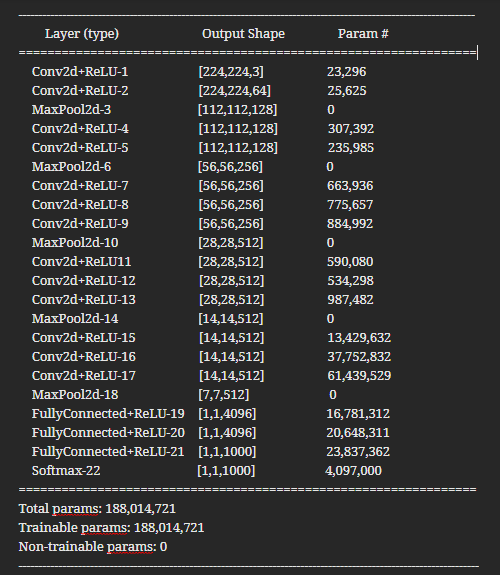
\includegraphics[scale=0.7]{Figures/object_summ.png}	
	\caption{Model summary of the text detection model}
	\label{fig:object_summ}
\end{figure}


\vspace{0.75cm}
 In  this chapter we saw that \acrlong{rcn} is faster in both training and testing and is much more efficient than the traditional methods like CNN (Convolutional Neural Networks) and OCR (Optical Character Recognition) for object detection and also the details of the model used to build the text detector.


%Chapter 4
\chapter{Denoising Autoencoder}

\indent\indent Denoising autoencoders are used to denoise an input image. They are widely used as first pre--processing step in various image processing applications. This chapter gives a brief introduction to denoising autoencoders. It further gives a description of our model summary and training details. 

\section{Autoencoding}
"Autoencoding" is a data compression algorithm where the compression and decompression functions are 1) data-specific, 2) lossy, and 3) learned automatically from examples rather than engineered by a human. These compression and decompression functions are usually implemented using neural networks.

\begin{enumerate}
\item Autoencoders are data-specific : they will only be able to compress data similar to what they have been trained on. An autoencoder trained on pictures of faces would do a rather poor job of compressing pictures of trees, because the features it would learn would be face-specific. Hence, one model cannot be generalised to all applications. They are application specific.
\item Autoencoders are lossy : the decompressed outputs will be degraded compared to the original inputs (similar to MP3 or JPEG compression). This differs from lossless arithmetic compression.
\item Autoencoders are learned automatically from data examples : it means that it is easy to train specialized instances of the algorithm that will perform well on a specific type of input. It doesn't require any new engineering, just appropriate training data.
\end{enumerate}
The aim of an autoencoder is dimensionality reduction and feature discovery. An autoencoder is trained to predict its own input,
but to prevent the model from learning the identity mapping,
some constraints are applied to the hidden units.\cite{yasenko2020image}
\vspace{0.75cm}

\section{\gls{da}}
Denoising autoencoders are an extension of simple autoencoders.  They add noise to inputs during a training process. Autoencoders are one of the unsupervised deep learning models. \cite{yasenko2020image} \\
Algorithm of \acrshort{da}:
\begin{enumerate}
    \item Manually adding noise, for our project, Gaussian Blur.
    \item Constructing an autoencoder model. It includes both encoding and decoding layers for compression and decompression respectively.
    \item Training the denoising autoencoder model on the noisy dataset. The reconstruction loss between the original image and its reconstruction obtained from final decoding layer is minimised in every epoch.
\end{enumerate}

% \ref{fig:autoencoder_schema} 
\begin{figure}[htb]
\centering
	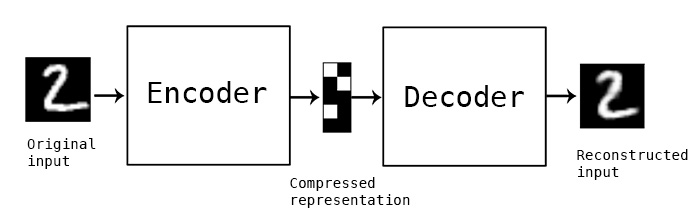
\includegraphics[scale=2.5]{Figures/autoencoder_schema}	
	\caption{Denoising Autoencoder}
	\label{fig:autoencoder_schema}
\end{figure}
\section{Software Setup}
\begin{enumerate}
\item Keras: Keras is an open-source software library that provides a python interface for artificial neural networks. Keras acts as an interface for the TensorFlow library.
\item PyCharm: PyCharm is an integrated development environment used in computer programming, specifically for the Python language.
\item Google Colab: Colaboratory, or “Colab” for short, is a product from Google Research. Colab allows anybody to write and execute arbitrary python code through the browser, and is especially well suited to machine learning, data analysis and education.
\end{enumerate}
\section{\gls{da} model summary}

% \ref{fig:denoise_model_summary} 
\begin{figure}[H]
\centering
	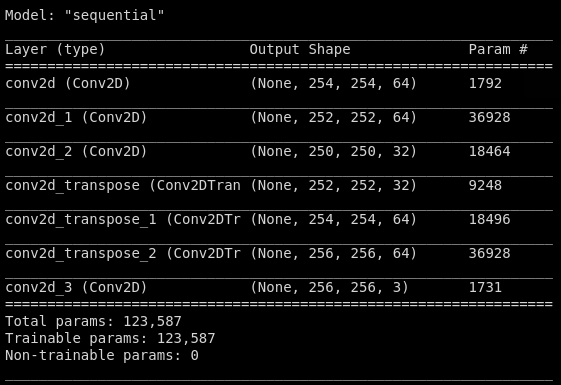
\includegraphics[scale=0.7]{Figures/denoise_model_summary.png}	
	\caption{Model Summary of \acrlong{da}}
	\label{fig:denoise_model_summary}
\end{figure}

\section{Training details}
The model is developed and trained using Keras framework with Tensorflow backend. The model has three convolution layers for encoding or compressing and three convolution transpose layers i.e. convolution $+$ upsampling, for decoding or decompressing as shown in figure \ref{fig:denoise_model_summary}. The last convolution layer is used to map the normalised pixel values between 0 and 1. To achieve this, sigmoid activation function is used which is given by \ref{c4:eqn1}.\\
% Choice of activation function and loss function:\\ 
% Sigmoid activation function is used in the last convolution layer to map the normalised pixel values to a value between 0 and 1. \\
% Sigmoid activation function is given by \ref{c4:eqn1}. 
\begin{equation}
\label{c4:eqn1}
\fontsize{12}{12}\selectfont
f(s_{i}) = \frac{1}{(1+e^{x})}
\end{equation}
% \ref{fig:Sigmoid} 
\begin{figure}[H]
\centering
	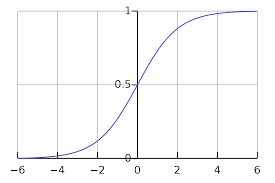
\includegraphics[scale=1]{Figures/sigmoid.png}	
	\caption{Sigmoid activation function}
	\label{fig:Sigmoid}
\end{figure}
The reconstruction loss is calculated for these mapped values using Binary Cross-Entropy Loss function (Sigmoid Cross-Entropy loss function), which is given by equations \ref{c4:eqn2} and \ref{c4:eqn3}.
\begin{equation}
\label{c4:eqn2}
\fontsize{12}{12}\selectfont
\begin{aligned}
\gls{ce} 
& = \sum_{i=1}^{c'=2}{(t_{i})\log(f(s_{i})))}\\
& = -{(t_{1})\log(f(s_{1}))} - ({1 - (t_{1}))\log(1 - f(s_{1}))}
\end{aligned}
\end{equation}

\begin{equation}
\label{c4:eqn3}
\fontsize{12}{12}\selectfont
\gls{ce} = 
\begin{cases}
  -\log(f(s_{1})) & if \hspace{5pt} t_{1} = 1 \\
  -\log(1 - f(s_{1})) & if \hspace{5pt} t_{1} = 0\\
\end{cases}
\end{equation}

To summarize, a denoising autoencoder is an image processing technique which is used to remove noise from an image. It has both downsampling and upsampling layers. In downsampling the model learns various features of the image and it reconstructs the image based on the learnt features in upsampling.

\begin{figure}[H]
\centering
	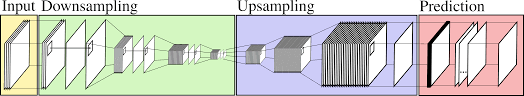
\includegraphics[scale=0.9]{Figures/denoise_summary.png}	
	\caption{\acrlong{da} summary}
	\label{fig:denoise_model_summary}
\end{figure}

%Chapter 5
\chapter{Text Extraction and Summarization}

\indent\indent The first part of this chapter gives a brief description of text extraction method used in our project and its internal working. The second part explains the text summarization algorithm.  
\section{Text extraction}
Optical Character Recognition (OCR) is the process of
converting any form of text or text-containing documents such as handwritten text, printed or scanned text images, into an editable digital format for deeper and further processing. \cite{hamad2016detailed}
Tesseract is an open source text recognition (OCR) Engine, available under the Apache 2.0 license. It can be used directly, or (for programmers) using an API to extract printed text from images. It can be used with the existing layout analysis to recognize text within a large document, or it can be used in conjunction with an external text detector to recognize text from an image of a single text line.\\
Tesseract 3.x was dependant on the multi-stage process:
\begin{enumerate}
    \item Word finding
    \item Line finding
    \item Character classification
\end{enumerate}

Word finding is done by organizing text lines into blobs, and the lines and regions are analyzed for fixed pitch or proportional text. Text lines are broken into words differently according to the kind of character spacing. Recognition then proceeds as a two-pass process. In the first pass, an attempt is made to recognize each word. Each word that is satisfactory is passed to an adaptive classifier as training data. The adaptive classifier then recognizes the text accurately.

Modernization of the Tesseract tool was an effort on code cleaning and adding a new LSTM (Long Short Term Memory networks) model. The input image is processed in boxes (rectangle) line by line feeding into the LSTM model and giving output. 

% \ref{fig:extract} 
\begin{figure}[H]
\centering
	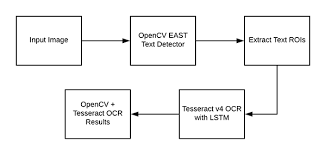
\includegraphics[scale=1]{Figures/extract.png}	
	\caption{Text extraction}
	\label{fig:extract}
\end{figure}

\section{Summarization}
Summarization \cite{reddy2012efficient} is the process of compressing the original document into a short summary by extracting the most important information from the document. The summary of the document can be helpful to the user to get the main theme of the document in a short span of time. The flow of information in a given document is not uniform, which means that some parts are more important than others. The important task in summarization lies in distinguishing the more informative parts of a document from the less ones.\\
Extractive vs. Abstractive summarization: 
\begin{enumerate}
    \item An extractive summarization method is the process of selecting most important sentences from the original document
    \item An abstractive summarization method produces a short summary by rephrasing the sentences that convey the same information. It involves natural language processing.\\ 
\end{enumerate}
Extractive summaries \cite{madhuri2019extractive} can be formulated by extracting the text segments (sentences or paragraphs) from the text based on the term frequency and sentence similarity. \\
There are several scenarios where automatic construction of summaries is useful. Other examples include automatic construction of summaries of news articles or email messages for sending them to mobile devices as SMS; summarization of information for government officials, business persons, researches, etc., and summarization of web pages to be shown on the screen of a mobile device, among many others. The Extraction based summarization methods will extracts the most important sentences from the given document. The main challenge of document summarization is to decide which sentences from the input document should be included in a summary. It first, assigns a score to each sentence and then gives ranks to the sentences according to their scores. The sentence with highest score will get the top rank. The score for a sentence is calculated by using statistical features including sentence position, cue words, term frequency, document frequency, topic signature, etc. \\
Text Summarization is the art of abstracting key content from information sources. Text summarization is one of the many applications of natural language processing and is becoming more popular for information condensation. Natural Language Processing played an important role developing the summary from a large extract. Concepts such as stemming and lemmatization was crucial in the development of the summary. Stemming ensures that all similar words are normalized while lemmatization ensures that infected words were mapped to their healthy dictionary forms. The summarization was done on the basis of eliminating less important sentences from the extract and concurrently keeping the more important ones. The usefulness of a sentence was judged based on the frequency of relevant words in it. The Natural Language Toolkit (NLTK) is used in our project for text summarization.\\
% \ref{fig:summarizer} 
\begin{figure}[H]
\centering
	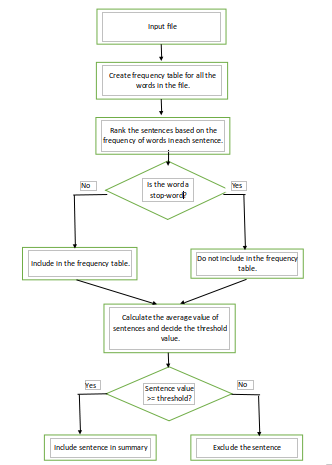
\includegraphics[scale=1]{Figures/summarizer.png}	
	\caption{Summarization Flow}
	\label{fig:summarizer}
\end{figure}


\vspace{0.75cm}
In summary, text extraction is a process of generating text from electronic documents that have associated text. The tesseract module of python uses OCR to extract text from images. Text summarization is a method of removing redundant information from text by using frequency tables. Natural language toolkit is used for achieving this.
  

%Chapter 6
\chapter{Results \& Discussions}
\indent\indent This chapter includes results obtained individually from object detection model, denoising autoencoder and text extraction, and the final result obtained after combining all models with text summarization. It also includes a text extraction and summarization comparison for pure and deblurred slide images.
\section{Object detection model}
This section includes training details, model accuracy and results obtained for object detection model.
\subsection{Training details}
% \ref{c6:tab1} Results of Object detection model
\begin{table}[H]
\centering
\fontsize{10}{12}\selectfont
\caption{Object detection Training}
\label{c6:tab1}
\small\addtolength{\tabcolsep}{40pt}
\def\arraystretch{1.5}
\begin{tabular}{|p{5cm}|p{2cm}|}
	\hline
% 	\multicolumn{2}{|c|}{Training} \\
	
% 	\hline
	\textbf{Number of epochs}   & 16000\\\hline
	\textbf{Training images used}&   320\\\hline
	\textbf{Validation images used} & 90\\\hline
	\textbf{Total loss}  &  0.035\\\hline
\end{tabular}
\end{table}
\subsection{Accuracy}
% \ref{fig:accuracy} 
\begin{figure}[H]
\centering
	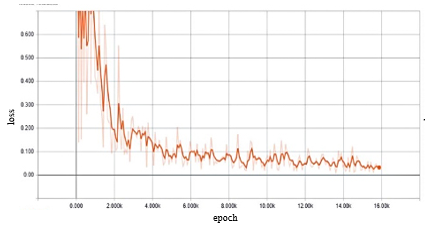
\includegraphics[scale=1]{Figures/ob_loss.png}	
	\caption{Object detection total loss}
	\label{fig:ob_loss}
\end{figure}

% \ref{fig:loss} 
\begin{figure}[H]
\centering
	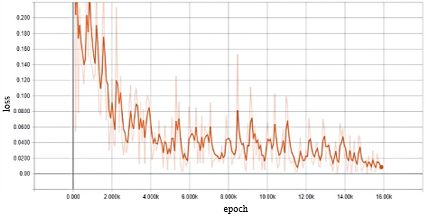
\includegraphics[scale=1]{Figures/ob_class.png}	
	\caption{Object detection classification loss}
	\label{fig:ob_class}
\end{figure}
\subsection{Result obtained}
% \ref{fig:detect1} 
\begin{figure}[H]
\centering
	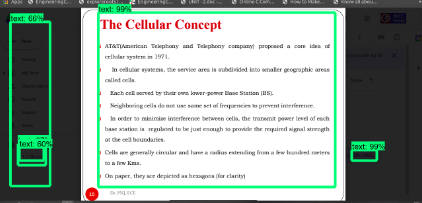
\includegraphics[scale=1]{Figures/detect1.png}	
	\caption{Object detection result}
	\label{fig:detect1}
\end{figure}

\section{Denoising Autoencoder}
This section includes training details, model accuracy and results obtained for denoising autoencoder.
\subsection{Training details}
\begin{table}[H]
\centering
\fontsize{10}{12}\selectfont
\caption{\acrlong{da} training}
\label{c6:tab2}
\small\addtolength{\tabcolsep}{40pt}
\def\arraystretch{1.5}
\begin{tabular}{|p{5cm}|p{2cm}|}
	\hline
% 	\multicolumn{2}{|c|}{Training} \\
	
% 	\hline
	\textbf{Number of epochs}   & 1000\\\hline
	\textbf{Training images used}&   280\\\hline
	\textbf{Validation images used} & 70\\\hline
	\textbf{Training accuracy}    &91\%\\\hline
	\textbf{Validation accuracy}&   87\%\\\hline
	\hline
\end{tabular}
\end{table}
\subsection{Training and validation accuracy}
% \ref{fig:accuracy} 
\begin{figure}[H]
\centering
	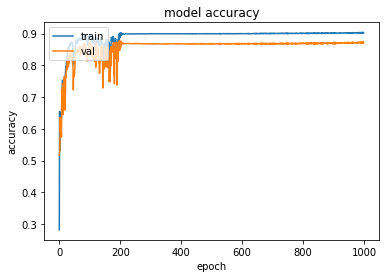
\includegraphics[scale=1]{Figures/denoise_accuracy.png}	
	\caption{\acrlong{da} Accuracy}
	\label{fig:denoise_accuracy}
\end{figure}
\subsection{Training and validation loss}
% \ref{fig:loss} 
\begin{figure}[H]
\centering
	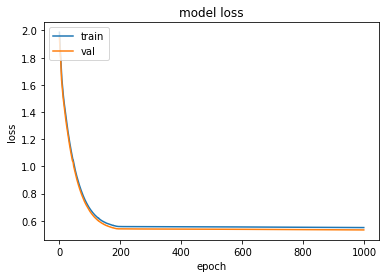
\includegraphics[scale=1]{Figures/denoise_loss.png}	
	\caption{\acrlong{da} Loss}
	\label{fig:denoise_loss}
\end{figure}
\subsection{Result obtained}
% \ref{fig:denoise} 
\begin{figure}[H]
\centering
	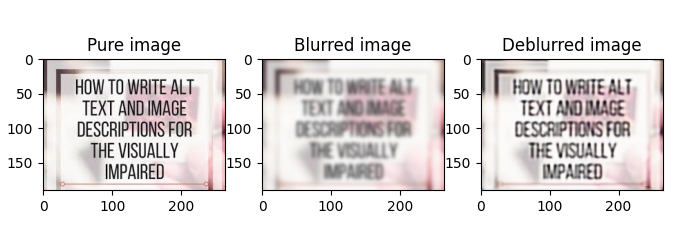
\includegraphics[scale=0.7]{Figures/denoise1.png}	
	\caption{\acrlong{da} output}
	\label{fig:denoise}
\end{figure}

\section{Text Extraction}
This section includes results obtained from text extraction method for a pure, blurred and deblurred image.
\subsection{Text extraction for pure image}
% \ref{fig:pure} 
\begin{figure}[H]
\centering
	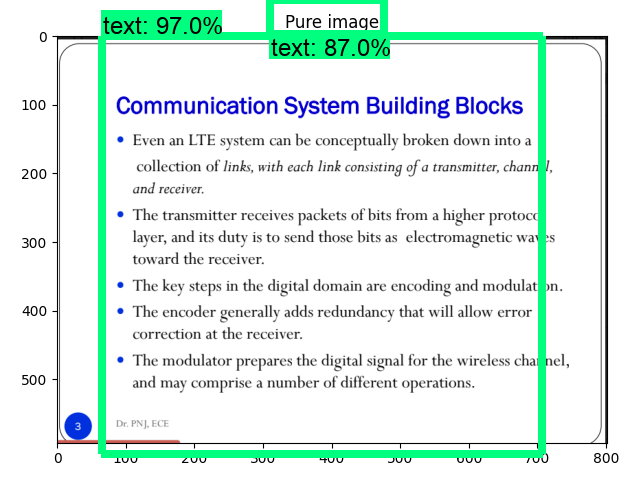
\includegraphics[scale=0.7]{Figures/myplot_pure.png}	
	\caption{Pure image}
	\label{fig:pure}
\end{figure}
% \ref{fig:pure_op} 
\begin{figure}[H]
\centering
	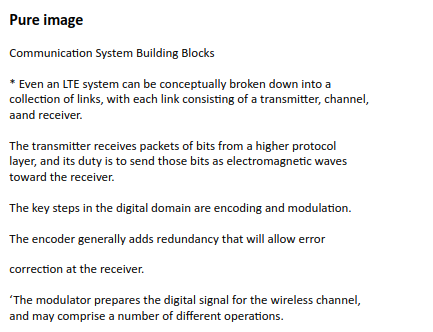
\includegraphics[scale=0.7]{Figures/pure_op.png}	
	\caption{Text Extracted from pure image}
	\label{fig:pure_op}
\end{figure}

\subsection{Text extraction for blurred image}
% \ref{fig:blur} 
\begin{figure}[H]
\centering
	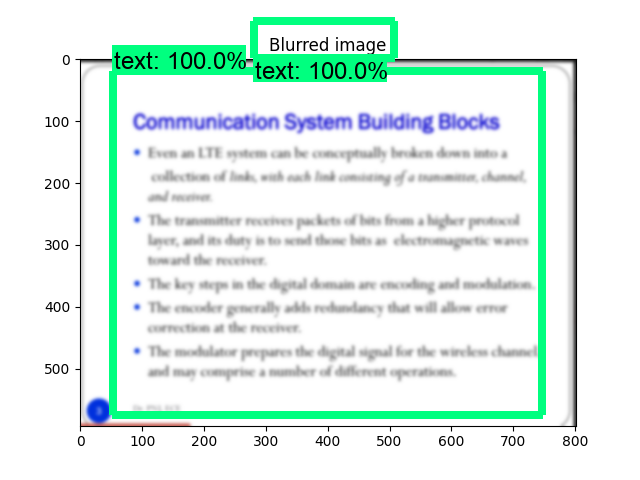
\includegraphics[scale=0.7]{Figures/myplot_blur.png}	
	\caption{Blurred image}
	\label{fig:blur}
\end{figure}
% \ref{fig:blur_op} 
\begin{figure}[H]
\centering
	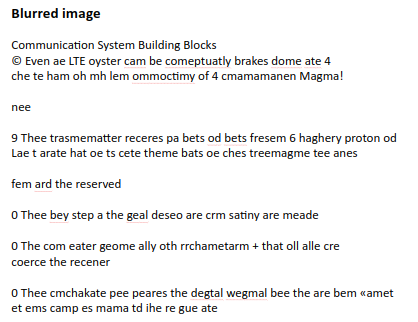
\includegraphics[scale=0.7]{Figures/blur_op.png}	
	\caption{Text Extracted from blurred image}
	\label{fig:blur_op}
\end{figure}

\subsection{Text extraction for deblurred image}
% \ref{fig:deblur} 
\begin{figure}[H]
\centering
	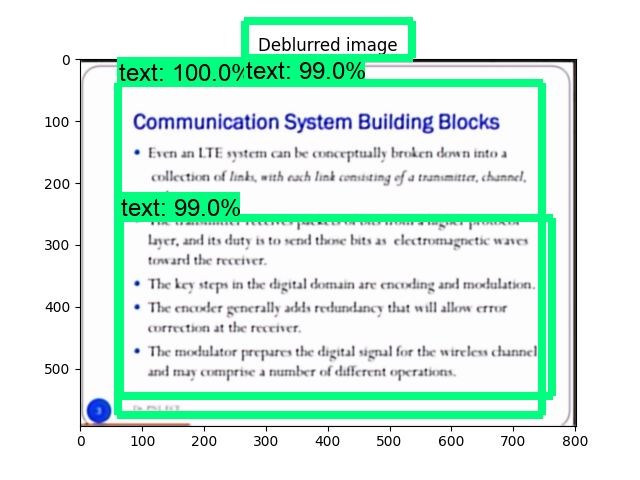
\includegraphics[scale=0.7]{Figures/myplot_deblur.png}	
	\caption{Deblurred image}
	\label{fig:deblur}
\end{figure}
% \ref{fig:deblur_op} 
\begin{figure}[H]
\centering
	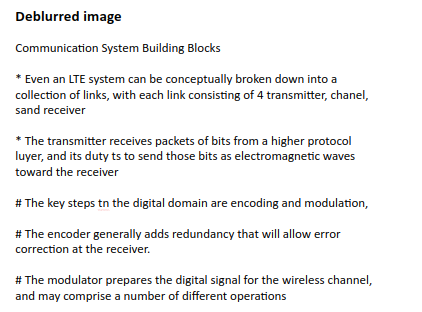
\includegraphics[scale=0.7]{Figures/deblur_op.png}	
	\caption{Text Extracted from deblurred image}
	\label{fig:deblur_op}
\end{figure}
\newpage
\section{Summarization}

\subsection{Summarization of text extracted from pure slides}
Extracted text from pure slides is shown in figure \ref{fig:orig_text2}.
\begin{figure}[H]
\centering
	\makebox[\textwidth]{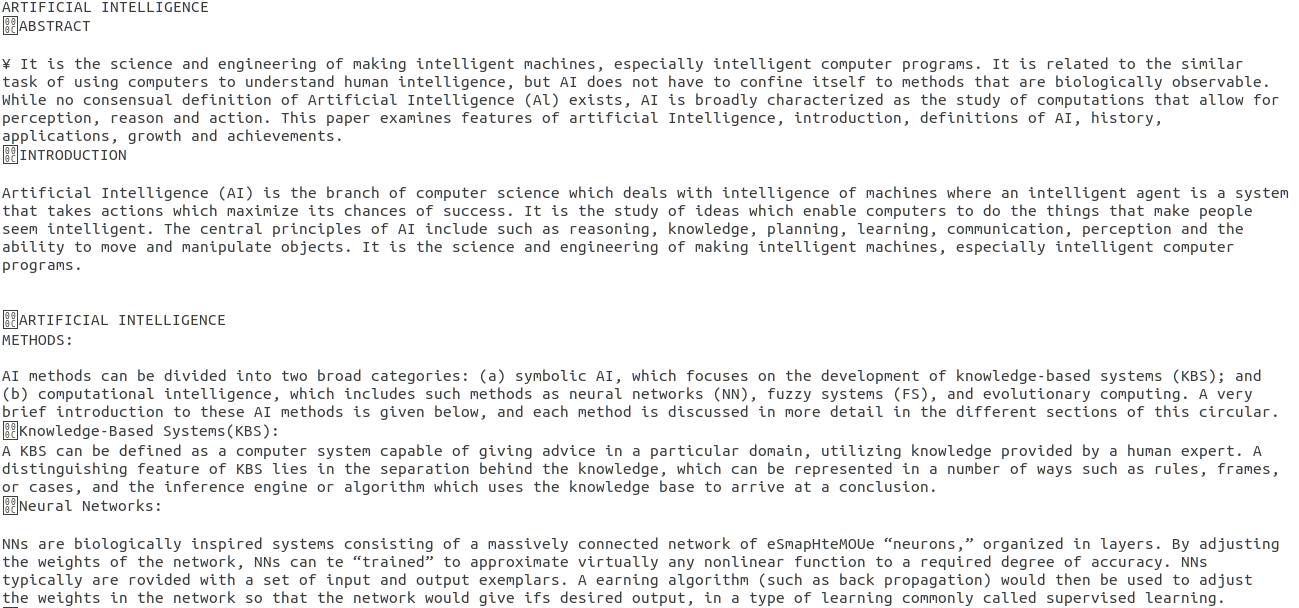
\includegraphics[scale=0.45]{Figures/orig_text1.png}}
% 	\caption{Text extracted from pure slides}
	\label{fig:orig_text1}
\end{figure}
% \ref{fig:deblur_op} 
\begin{figure}[H]
\centering
	\makebox[\textwidth]{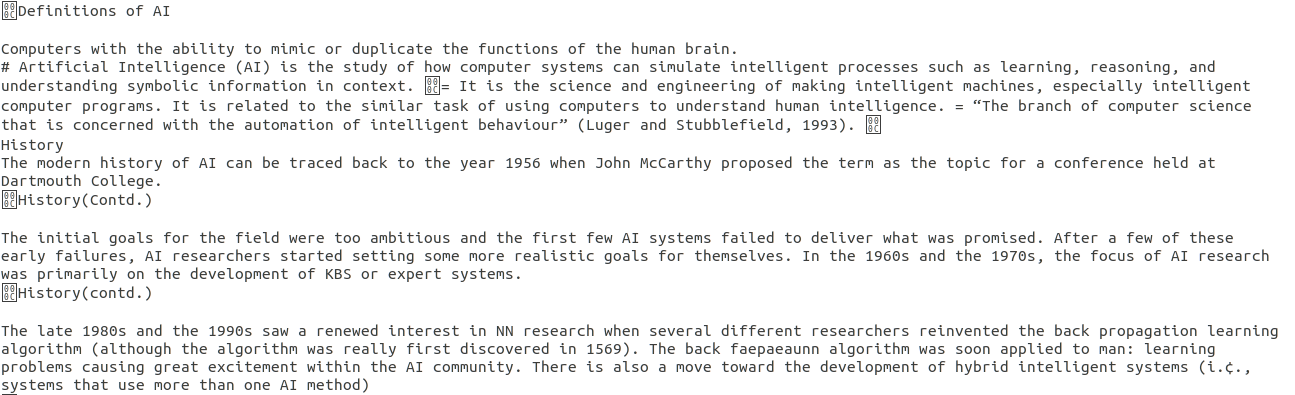
\includegraphics[scale=0.45]{Figures/orig_text2.png}}	
	\caption{Text extracted from pure slides}
	\label{fig:orig_text2}
\end{figure}
\newpage
Summary generated for the above text is shown in figure \ref{fig:orig_sum1}.
\begin{figure}[H]
\centering
	\makebox[\textwidth]{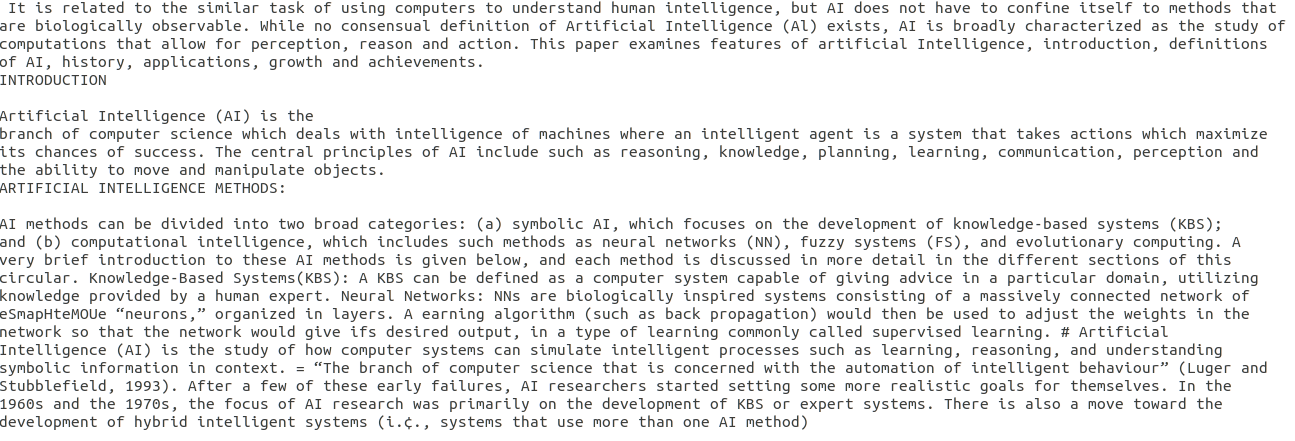
\includegraphics[scale=0.45]{Figures/orig_sum1.png}}	
	\caption{Text summarized from pure slides}
	\label{fig:orig_sum1}
\end{figure}

\subsection{Summarization of text extracted from deblurred slides}
Extracted text from deblurred slides is shown in figure \ref{fig:deblur_text2}.
\begin{figure}[H]
\centering
	\makebox[\textwidth]{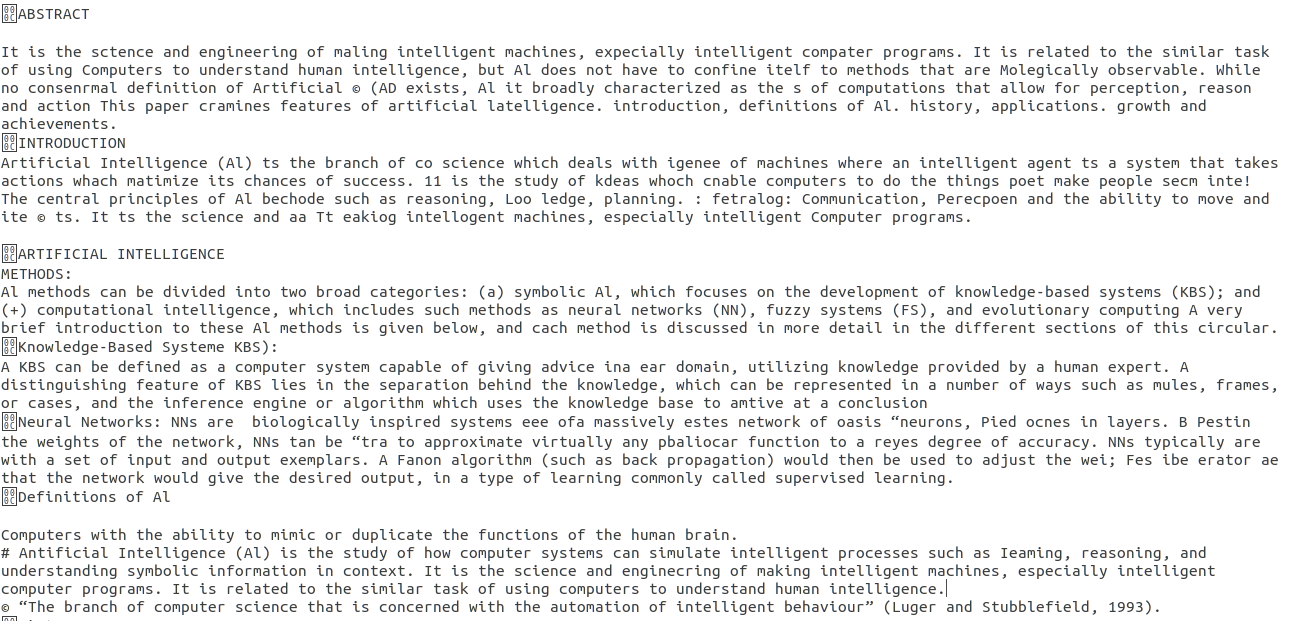
\includegraphics[scale=0.45]{Figures/deblur_text1.png}}
% 	\caption{Text extracted from pure slides}
	\label{fig:deblur_text1}
\end{figure}
% \ref{fig:deblur_op} 
\begin{figure}[H]
\centering
	\makebox[\textwidth]{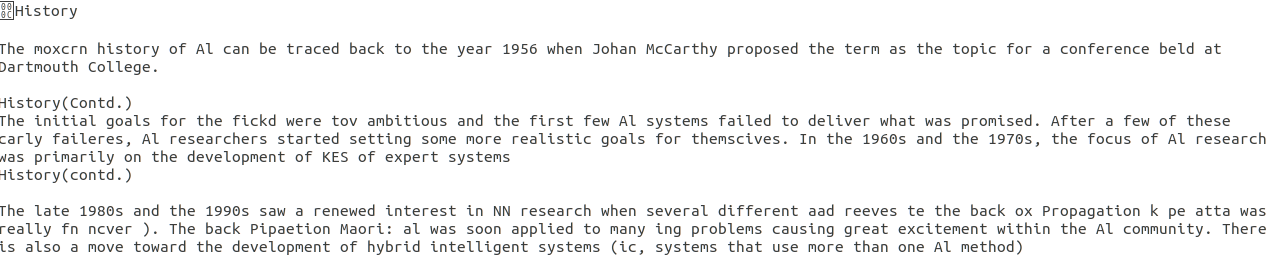
\includegraphics[scale=0.45]{Figures/deblur_text2.png}}	
	\caption{Text extracted from deblurred slides}
	\label{fig:deblur_text2}
\end{figure}
% \newpage
Summary generated for the above text is shown in figure \ref{fig:deblur_sum1}.
\begin{figure}[H]
\centering
	\makebox[\textwidth]{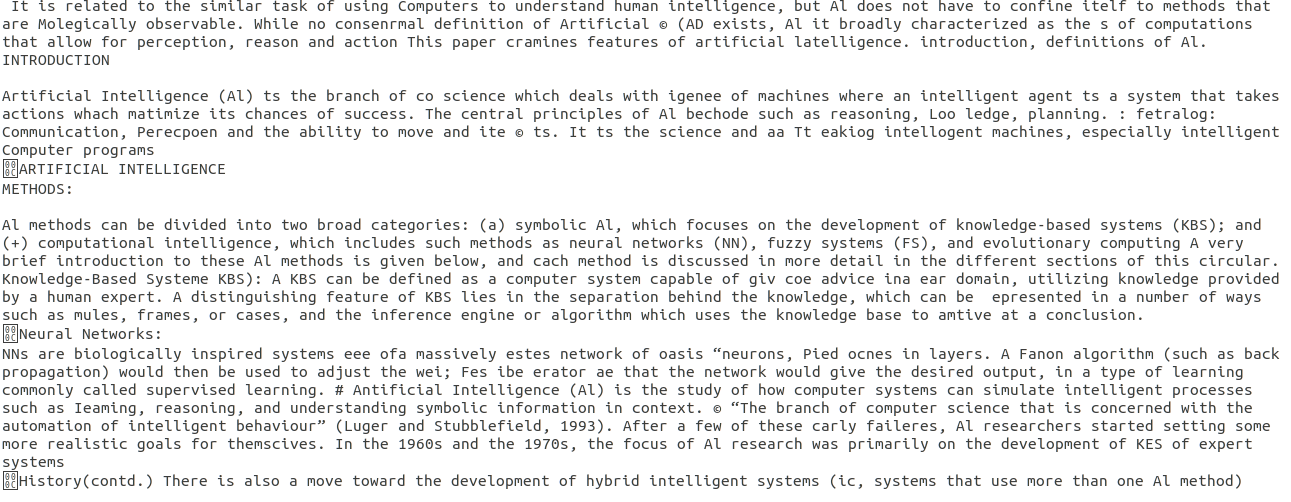
\includegraphics[scale=0.45]{Figures/deblur_sum1.png}}	
	\caption{Text summarized from deblurred slides}
	\label{fig:deblur_sum1}
\end{figure}

To summarize, this chapter gives independent results obtained for each trained model. Final section gives the result obtained after combining all the models. It also gives a comparison of results obtained for pure, blurred and deblurred images where deblurring is achieved using denoising autoencoder.






%Chapter 7
\chapter{Conclusion and Future Scope}

\section{Conclusion}

This project provides a smart solution of summarizing the entire presentation and logging it. There are two main objectives of this project. The first objective of this project is to build a more efficient object detection model compared to OCR (Optical Character Recognition) since OCR has many drawbacks associated with it such as reduced accuracy when input images are skewed or have low lighting. The second one is to extract text from blurred images and summarize the same. 

The first objective was met by implementing a faster \acrshort{rcn} model for text detection. This model is proven to have better accuracy compared to OCR. The second objective was met by developing a denoising autoencoder which will deblur an image before passing it through the object detection model. This ensures better extraction efficiency. 

An efficient faster \acrshort{rcn} model was developed for text detection which yielded a total loss of only 0.035. Denoising autoencoder was successfully developed and trained to obtain a training accuracy of 91\% and a validation accuracy of up to 87\%. This accuracy can be further improved by training the model on a larger dataset for more number of epochs.
% First paragraph should bring in the scenario of the project and every objective should be explained here.

% Second paragraph should say how the objectives are implemented and achieved.

% Last paragraph should draw the conclusions from each objective with quantitative results, performance improvement etc. 

\section{Future Scope}
The future scope of the project should not limit its usage to classrooms or small presentations, but should be able to extend its capability, to cater to larger presentations and seminars. In order to achieve better quality text detection, an area that can be addressed would be recording the audio and integrating the audio and images to get a detailed summary. Noise may persist in the case of lower-grade equipment or even improper placement of the device on uneven terrain. Noise detection can improve the scope of use of this product. The microphone is extremely susceptible to external interference from the surroundings. To address this issue, better-grade equipment can be installed in the audio interface. Another solution is to ensure that the speaker, or the person making the delivery has a personalized microphone specifically for this purpose. \\

Another extension that can be made is to generate personalized summaries specific to each user. A user who has paid more attention to the delivery or has prior knowledge of the topic, may not need as detailed a summary as to someone who has paid less attention or someone who is not well--versed in that particular field. The personalization can be used to cater to these specific needs.

\section{Learning Outcomes of the Project}
Over the course of the project, many concepts and tools were learnt, and the project was built successfully.
\begin{itemize}
\item Domains like Image Processing and machine learning, were explored in good depth in this project.
\item We were able to understand the working of CNNs and extend its implementation to object detection model and denoising autoencoder.
\item We were able to identify hardware limitations for training the models and overcome the problems that they might cause by implementing optimization methods like L2 regularization.
\item We understood the concepts of Natural Language Processing, and applied them successfully to get the summary of the extracted text.
\item We were able to identify its shortcomings for industrial applicability and address some of those issues in this report.

\end{itemize}



\backmatter
\clearpage
%\ifDrft{
%%Do Nothing
%}\else{
\printbibliography%
%}
%\printindex
\end{spacing}
\end{document}